%!TEX root = ../thesis.tex
\section{Design Guidelines}

To motivate and inform the design of a tool to support live presentations, we collected preferences for software demonstrations using an online survey. We describe the three design goals derived from the survey results.

\subsection{Understanding Demo Preferences} To understand both presenters' and audiences' preferences for performing and viewing system demonstrations, we conducted an online survey in a software company and a university research lab. Our goal was to collect people's feedback on giving and seeing software demonstrations during live presentations. We received 73 responses from researchers, graduate students, software engineers, and designers. Their main research areas include human-computer interaction (64.4\%), software engineering (21.9\%), and machine learning (20.6\%); 66.7\% were male. Among all the respondents, 35.6\% indicated that they were very experienced at giving software demos to the audience during a live presentation; 46.6\% had demoed at least once; 13.7\% had not demoed but attended talks that showed a software demonstration.

We asked respondents who had demo experience (\textit{N} = 60) how they preferred to perform a demo. Their answers were: a live demo (25 out of 60), pre-recorded videos (15), a mixed format of a live demo and videos (12), static screenshots (4), and other (4). In Table~\ref{tab:demowiz_survey}, we list the top 2-3 reasons for their preferences. Giving a \textit{live demo} can be more engaging with a working system and match the audience's interests, but presenters can encounter unexpected problems and forget to show important features within a given time constraint. On the other hand, presenting with \textit{a demo video} avoids such problems by extracting the most important parts, and can allow visual highlighting (labeling or zooming), but can be less engaging. In addition, it is hard to narrate.

We were also interested in reactions as an audience member. For respondents who had seen software demos (\textit{N} = 70), we asked how they preferred to see the demonstration performed. We found a slightly different preference: a live demo (36 out of 70), a mixed format of a live demo and videos (24), pre-recorded videos (7), and other (3). However, the reasons were well aligned with presenters’ concerns. A\textit{ live demo} shows a working system and can be more engaging, but the audience might need to wait for system problems to be resolved or sometimes see presenters rambling. A\textit{ demo video }can show the most important parts, sometimes assisted by visual highlighting, but it can be hard to tell which parts of a demo are real, and can be less engaging to the audience.

\subsection{Design Goals} From the survey results, we understand that giving a live demo is often more preferable than showing demo videos. However, we cannot, in general, address some of the main concerns with giving a live demo – that is, stability of the software system and variations in the presentation environment which can cause the demo to fail. Therefore, we instead aim to address some of the drawbacks with demo videos while preserving their advantages. More specifically, our goal is to make demo videos \textit{more engaging} by assisting presenters in adjusting their narration to guide the audience through the material. In this section, we describe our design goals to support more effective demo video presentations.

\subsubsection{G1. Show what's coming next, where and when it will occur.}
To engage the audience with the demonstration, it is important for presenters to guide the audience's attention to the right place at the right time. To do so, presenters should be fully aware of upcoming actions – specifically \textit{what} actions will happen, \textit{where} they will occur on the screen, and \textit{when} they will happen.

\subsubsection{G2. Minimize required attention or interpretation.}
While it is our desire to help presenters understand and anticipate impending events, we should not overburden a presenter who is already narrating a specific set of talking points. As a tradeoff between providing more information and minimizing cognitive load, any augmentation of the video needs to be offered in a glanceable fashion, i.e., information can be interpreted quickly and without the presenter's full attention.

\subsubsection{G3. Support light-weight editing during rehearsal.}
Different presentations may require more or less extensive explanations, and when first recording a demo video, it may not be possible to perform the demo at the same rate necessary for a live presentation (e.g., typing can be difficult or system response times may be variable). In addition, it should be easy to review, practice, and modify the pace for a particular presentation. For all these reasons, lightweight editing and rehearsal are necessary.  Using these principles as a guiding rubric for our design, we iterated on several versions of the DemoWiz system.

\begin{table}
  \centering
  % 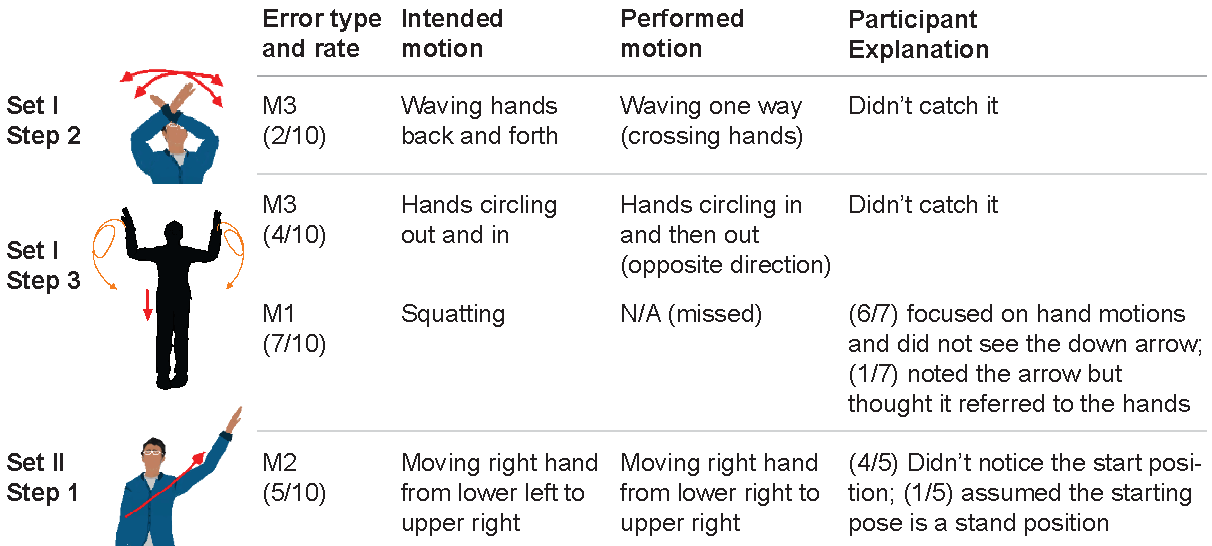
\includegraphics[width=\columnwidth]{\demodraw/fig/study1/study1}
  \caption{Survey of software demonstration preferences from presenters' (N=60) and audience's (N=70) point of views.}
  \label{tab:demowiz_survey}
\end{table}
